% gm-07-Factoring.tex

\documentclass[xcolor=dvipsnames]{beamer}

\usepackage{cancel}
\renewcommand{\CancelColor}{\color{red}}
\usepackage{graphicx}
\usepackage{wrapfig}
\usepackage{colortbl}
\usepackage{color}
\usepackage{alltt}
\renewcommand*{\thefootnote}{\fnsymbol{footnote}}
\definecolor{myblue}{rgb}{0.8,0.85,1}

\mode<presentation>
{
  \usetheme{Warsaw}
  \setbeamercovered{transparent}
}
% \usecolortheme[named=OliveGreen]{structure}
\setbeamertemplate{navigation symbols}{} 
\setbeamertemplate{blocks}[rounded][shadow=true] 

% this is for overlaying math symbols, see https://tex.stackexchange.com/questions/12895/overlay-symbol-with-another
\def\qeq{\mathrel{%
    \mathchoice{\QEQ}{\QEQ}{\scriptsize\QEQ}{\tiny\QEQ}%
}}
\def\QEQ{{%
    \setbox0\hbox{$\longrightarrow$}%
    \rlap{\hbox to \wd0{\hss/\hss}}\box0
  }}

\newcounter{expls}
\setcounter{expls}{0}
\newcommand{\beispiel}[1]{\refstepcounter{expls}\textbf{Example \arabic{expls}: #1.}}

\newcounter{exercise}
\setcounter{exercise}{0}
\newcommand{\ubung}[0]{\refstepcounter{exercise}\textbf{Exercise \arabic{exercise}: }}

\newif\ifBCITCourse
\BCITCoursetrue
% \BCITCoursefalse
\newif\ifWhichCourse
\WhichCoursetrue
\WhichCoursefalse
\ifBCITCourse
\ifWhichCourse
\newcommand{\CourseName}{Technical Mathematics for Food Technology}
\newcommand{\CourseNumber}{MATH 1441}
\newcommand{\CourseInst}{BCIT}
\else
\newcommand{\CourseName}{Technical Mathematics for Geomatics}
\newcommand{\CourseNumber}{MATH 1511}
\newcommand{\CourseInst}{BCIT}
\fi
\else
\newcommand{\CourseName}{Philosophy and Literature}
\newcommand{\CourseNumber}{PHIL 375}
\newcommand{\CourseInst}{UBC}
\fi

\title{Factoring}
\subtitle{{\CourseNumber}, BCIT}

\author{\CourseName}

\date{October 11, 2017}

\begin{document}

\begin{frame}
  \titlepage
\end{frame}

\begin{frame}
  \frametitle{Three Types of Factoring}
In this unit, we will address three types of factoring.
\begin{enumerate}
\item Common Terms
\item Difference of Squares
\item Quadratic Equation
\end{enumerate}
The idea is to be skilled in both directions, \alert{factoring} and
\alert{expanding}.
  \begin{figure}[h]
    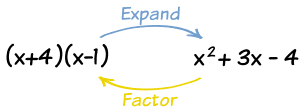
\includegraphics[scale=1]{./factorexpand.png}
  \end{figure}
\end{frame}

\begin{frame}
  \frametitle{Common Terms}
Factor out the common terms and simplify.
\begin{equation}
  \label{eq:yohpeumo}
3x-6x^{2}  
\end{equation}
\begin{equation}
  \label{eq:eeviewie}
  3x^{2}y-6x^{2}y
\end{equation}
\begin{equation}
  \label{eq:eewahque}
  \frac{80p^{3}-60pq^{3}}{80pq}
\end{equation}
\begin{equation}
  \label{eq:seeyeede}
  \frac{80p^{3}-60pq^{3}}{80+pq}
\end{equation}
\end{frame}

\begin{frame}
  \frametitle{Difference of Squares}
Always have the following three identities at your fingertips.
\begin{equation}
  \label{eq:ooheetae}
  a^{2}-b^{2}=(a-b)(a+b)
\end{equation}
\begin{equation}
  \label{eq:phiecief}
  (a+b)^{2}=a^{2}+2ab+b^{2}
\end{equation}
\begin{equation}
  \label{eq:aingaixo}
  (a-b)^{2}=a^{2}-2ab+b^{2}
\end{equation}
\end{frame}

\begin{frame}
  \frametitle{Difference of Squares Exercises}
Factor the following expressions,
\begin{equation}
  \label{eq:gaiphahg}
x^{2}-4  
\end{equation}
\begin{equation}
  \label{eq:vaecutha}
49-P^{4}  
\end{equation}
\begin{equation}
  \label{eq:woobiedo}
12-t^{2}  
\end{equation}
\begin{equation}
  \label{eq:aashiech}
5q^{3}-125q  
\end{equation}
\begin{equation}
  \label{eq:shioreey}
28x^{2}-700y^{2}
\end{equation}
\begin{equation}
  \label{eq:ohpeefio}
r^{8}-1
\end{equation}
\end{frame}

\begin{frame}
  \frametitle{Quadratic Equations I}
  When we learned about quadratic equations, we found that completing
  the square will give us the solution to a quadratic equation.
  Consider the equation $2x^{2}-5x-3=0$.
  \begin{figure}[h]
    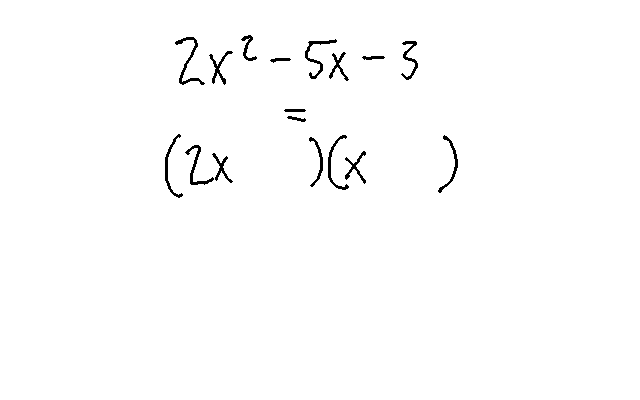
\includegraphics[scale=.4]{./qfac1.png}
  \end{figure}
\end{frame}

\begin{frame}
  \frametitle{Quadratic Equations I}
  When we learned about quadratic equations, we found that completing
  the square will give us the solution to a quadratic equation.
  Consider the equation $2x^{2}-5x-3=0$.
  \begin{figure}[h]
    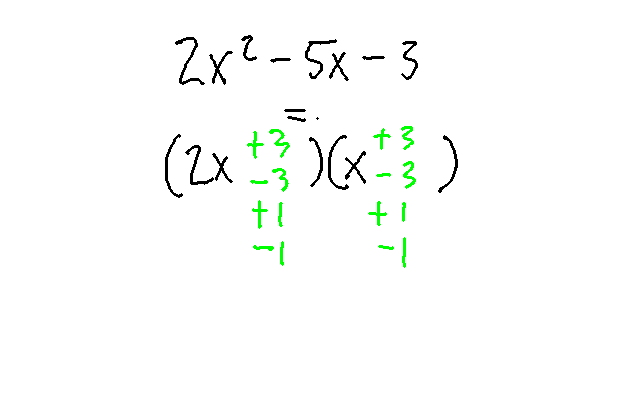
\includegraphics[scale=.4]{./qfac2.png}
  \end{figure}
\end{frame}

\begin{frame}
  \frametitle{Quadratic Equations I}
  When we learned about quadratic equations, we found that completing
  the square will give us the solution to a quadratic equation.
  Consider the equation $2x^{2}-5x-3=0$.
  \begin{figure}[h]
    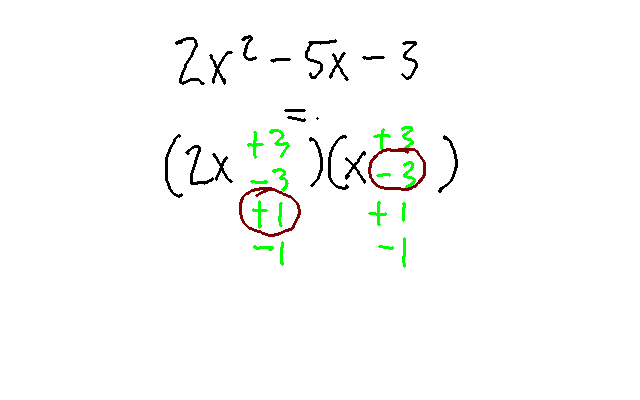
\includegraphics[scale=.4]{./qfac3.png}
  \end{figure}
\end{frame}

\begin{frame}
  \frametitle{Quadratic Equations I}
  When we learned about quadratic equations, we found that completing
  the square will give us the solution to a quadratic equation.
  Consider the equation $2x^{2}-5x-3=0$.
  \begin{figure}[h]
    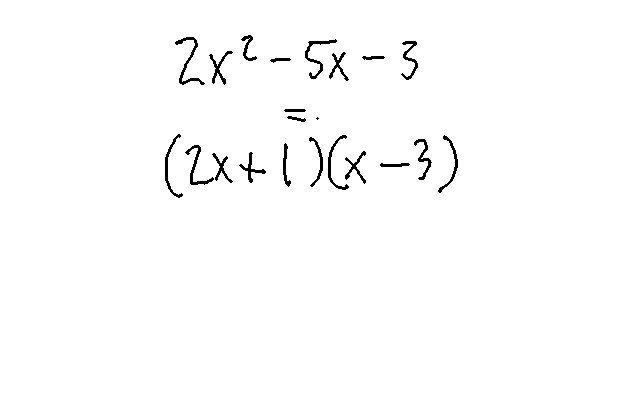
\includegraphics[scale=.4]{./qfac4.png}
  \end{figure}
\end{frame}

\begin{frame}
  \frametitle{Quadratic Equations I}
  When we learned about quadratic equations, we found that completing
  the square will give us the solution to a quadratic equation.
  Consider the equation $2x^{2}-5x-3=0$.
  \begin{figure}[h]
    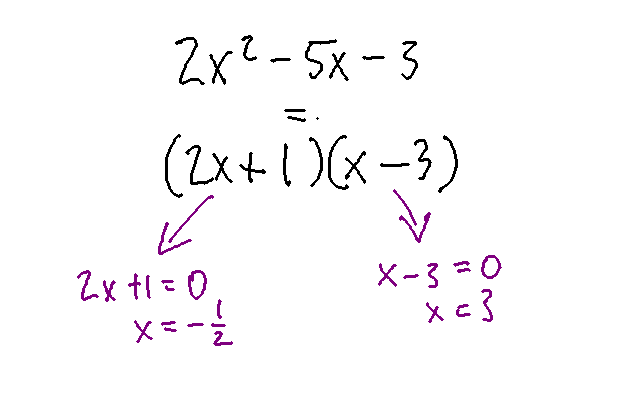
\includegraphics[scale=.4]{./qfac5.png}
  \end{figure}
\end{frame}

\begin{frame}
  \frametitle{Quadratic Equations I}
  When we learned about quadratic equations, we found that completing
  the square will give us the solution to a quadratic equation.
  Consider the equation $2x^{2}-5x-3=0$.
  \begin{figure}[h]
    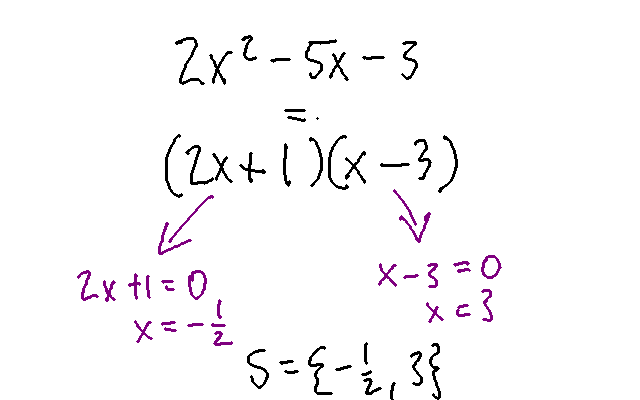
\includegraphics[scale=.4]{./qfac6.png}
  \end{figure}
\end{frame}

\begin{frame}
  \frametitle{Quadratic Equations II}
  Now that we want to factor a quadratic polynomial we could use the
  reverse procedure to find the factors. Instead of completing the
  square to find the solutions we could use the quadratic formula in
  order to find out how to complete the square. 
\begin{equation}
  \label{eq:aivaquie}
2x^{2}-5x-3=0
\end{equation}
\begin{equation}
  \label{eq:aiviaquo}
x_{1,2}=\frac{5\pm\sqrt{25-4\cdot{}2\cdot(-3)}}{2\cdot{}2}
\end{equation}
\begin{equation}
  \label{eq:achohgeo}
S=\left\{-\frac{1}{2},3\right\}
\end{equation}
\begin{equation}
  \label{eq:phopiini}
2x^{2}-5x-3=2\cdot(x-x_{1})(x-x_{2})=(2x+1)(x-3)
\end{equation}
\end{frame}

\begin{frame}
  \frametitle{Simplify by Factoring}
% Sullivan, page 636, 67--78
{\ubung} Simplify.
\begin{equation}
  \label{eq:lohsiela}
\frac{3x-6}{5x}\cdot\frac{x^{2}-x-6}{x^{2}-4}
\end{equation}
\begin{equation}
  \label{eq:aexoorai}
\frac{9x^{2}-25}{2x-2}\cdot\frac{1-x^{2}}{6x-10}
\end{equation}
\begin{equation}
  \label{eq:saevoyei}
  \frac{x}{x^{2}-7x+6}-\frac{x}{x^{2}-2x-24}
\end{equation}
\begin{equation}
  \label{eq:aijielio}
\frac{x}{(x-1)^{2}}+\frac{2}{x}-\frac{x+1}{x^{3}-x^{2}}
\end{equation}
\begin{equation}
  \label{eq:zohqueeh}
\frac{1}{h}\left(\frac{1}{(x+h)^{2}}-\frac{1}{x^{2}}\right)
\end{equation}
\end{frame}

\begin{frame}
  \frametitle{End of Lesson}
Next Lesson: Radians.
\end{frame}

\end{document}
